\documentclass[conference]{IEEEtran}
\IEEEoverridecommandlockouts
\usepackage[T1]{fontenc}
\usepackage{newtxtext,newtxmath}
\usepackage{booktabs,graphicx,array,tabularx,xcolor,tikz,enumitem}
\usepackage[hidelinks]{hyperref}
\usetikzlibrary{positioning,arrows.meta,fit}
\setlist{nosep,leftmargin=*}
\newcommand{\commitsha}{code and evidence commit \texttt{b6b09c23f6126766dbd794e5247d162807288dcf}}
\newcommand{\repo}{\url{https://github.com/zaki-cs25/Dat-Project}}
\newcommand{\tagurl}[1]{\href{https://github.com/zaki-cs25/Dat-Project/tree/cs5903-final-2026/#1}{\texttt{\detokenize{#1}}}}

\begin{document}

\title{Workload-Driven Evaluation of Self-Hosted LLM Serving: Precision, KV-Cache Quantization and Model Size under Agentic Traffic}

\author{\IEEEauthorblockN{Zaki Kazi (CS25MTECH11021)}
\IEEEauthorblockA{CS5903 Distributed AI Training, IIT Hyderabad\\
Project ID 24, Group 25\\
Repository: \repo\\
Tag \texttt{cs5903-final-2026}, \commitsha}}

\maketitle

\renewcommand{\abstractname}{Executive summary}
\begin{abstract}
An agent runs several dependent model calls per task, each carrying long context, so serving choices that win on flat benchmarks may not pay off for agent traffic. We compared six self-hosted serving setups on one NVIDIA A100 80\,GB while holding a real healthcare agent and a fixed 100-case workload constant: weight precision (BF16, Q8\_0), KV-cache precision (default, q8\_0), engine (vLLM, llama.cpp) and model size (Qwen3.6-27B, Qwen3-8B). Within llama.cpp each pair isolates one variable; vLLM--llama.cpp comparisons change engine and precision together. The agent interviews a patient, assesses urgency and drafts a retrieval-augmented care plan (about eight model calls, 23k input tokens per case); an independent LLM judge grades every completed plan against 500 weighted criteria. Qwen3.6-27B in BF16 on vLLM was the best deployment: 86/100 plans passed at INR\,2.97 per passed plan. Q8\_0 on llama.cpp was 42\% slower with 77--80 passes; a q8\_0 KV cache gave no speed benefit. Qwen3-8B halved latency but passed 44--53 plans: 16--22 plans per setup failed validation (mostly unknown citation identifiers) and the rest scored lower. An insurance agent showed the same model-size gap. \emph{Completion state:} all planned healthcare measurements are complete and graded; every reported number is regenerated from the raw outputs in the repository.
\end{abstract}

\section{Problem, scope and success criteria}
\textbf{Users and actors.} Operators who self-host an open-weight model for an agentic application; in the healthcare workload, the agent's users are patients (adaptive intake interview) and clinicians (read-only care-plan drafts).

\textbf{Problem.} Agent traffic differs from chatbot traffic: each task makes several dependent calls, context is long and repeated, and outputs must satisfy strict formats. Serving optimizations are usually evaluated on flat benchmarks with a fixed prompt shape. The question is: \emph{for a real agentic workload, which serving choices pay off, and what do they cost in answer quality?} Performance is never reported without quality, and cost is reported per useful answer.

\textbf{In scope.} Care-plan quality and serving performance over the full agent request path (four interview turns, assessment, care-plan generation, semantic review); serving variables model size, weight precision, KV-cache precision and engine. A second workload, insurance claim adjudication, checks model choice on a different traffic shape. \textbf{Out of scope.} Interview and triage quality scoring, clinical validation, prescribing (the agent never proposes diagnoses, drugs, doses or regimen changes) and multi-GPU serving.

\textbf{Assumptions and constraints.} One A100 80\,GB on a Slurm cluster whose QOS allows one GPU job per user, so setups run one after another; synthetic data only; a local embedding server.

\textbf{Milestones and frozen acceptance tests.} Not applicable: approved milestone IDs were not assigned to this project. The project's own acceptance tests and their observed status are in Table~\ref{tab:accept}.

\begin{table}[t]
\caption{Acceptance tests: expected vs observed}
\label{tab:accept}
\centering\scriptsize
\begin{tabularx}{\columnwidth}{@{}>{\raggedright\arraybackslash}p{2.0cm}>{\raggedright\arraybackslash}X>{\raggedright\arraybackslash}p{1.75cm}@{}}
\toprule
Test (done when) & Observed & Evidence \\
\midrule
End to end: interview yields assessment and FHIR \texttt{CarePlan} via the API & Met: every benchmark case runs registration $\rightarrow$ 4 interview turns $\rightarrow$ assessment $\rightarrow$ care-plan job through the API; 600 cases & run \texttt{cases.csv} \\
Protocol validity: all input, profile and trace hashes verified & Met: protocol valid, 100/100 checks verified in all six runs & \texttt{manifest.json} \\
Comparability: same dataset, agent image, sampling, judge & Met: dataset SHA identical; one agent image (ID recorded); same sampling; same judge model, prompt and rubrics & Sec.~\ref{sec:method} \\
Quality: every completed plan sent to the judge; no valid grade counts as not passed & Met: 99, 95, 97, 82, 80, 77 valid grades; the rest count as not passed & grade revisions \\
Metrics reported for every setup & Met & Tables~\ref{tab:health}--\ref{tab:serving} \\
Software tests pass & Met: 325 passed, 1 skipped; UI production build passes & logs in \texttt{evaluation/} \texttt{tests/} \\
\bottomrule
\end{tabularx}
\end{table}

\textbf{Changes from the approved mid-semester plan.} All changes in Table~\ref{tab:plan} were made in consultation with, and approved by, the course instructor; each has a decision record.

\begin{table}[t]
\caption{Changes from the mid-semester plan}
\label{tab:plan}
\centering\scriptsize
\begin{tabularx}{\columnwidth}{@{}>{\raggedright\arraybackslash}p{2.0cm}>{\raggedright\arraybackslash}X>{\raggedright\arraybackslash}p{0.75cm}@{}}
\toprule
Mid-semester plan & Delivered & ADR \\
\midrule
Serving matrix measured on insurance first & Full serving matrix measured on healthcare; insurance compares models & H08 \\
30-case healthcare set & 100-case CarePlan100 & H03 \\
vLLM for all setups & BF16 on vLLM, GGUF quantization on llama.cpp & H07 \\
Token-priced cost & GPU-time cost (INR per A100-hour) & H09 \\
Amount correct within 2\% & Within 1\% and exact (harness scorer) & I02 \\
1{,}000-case insurance run & 120-case golden set, 30 per verdict & I01 \\
\bottomrule
\end{tabularx}
\end{table}

\section{Related work, baselines and alternatives}
\textbf{Serving engines.} vLLM introduced PagedAttention for KV-cache memory management and continuous batching~\cite{kwon2023vllm}. llama.cpp serves GGUF models with integer weight formats such as Q8\_0 and supports quantized KV caches~\cite{llamacpp}. SGLang's RadixAttention targets prefix reuse in multi-call LLM programs, the traffic pattern agents produce~\cite{zheng2024sglang}.
\textbf{Quantization.} Weight-only 8-bit formats reduce memory and bandwidth with small quality loss; KV-cache quantization (e.g.\ KIVI~\cite{liu2024kivi}) reduces the memory of long contexts.
\textbf{Evaluation.} LLM-as-a-judge grading with explicit criteria is established for open-ended output~\cite{zheng2023judge}; rubric-based health evaluation is used by HealthBench~\cite{arora2025healthbench}. AMEGA evaluates guideline adherence of medical LLMs~\cite{fast2024amega}.

\textbf{Approaches considered} (details in the ADR log):
\begin{enumerate}
\item \emph{Flat synthetic load} (fixed prompt shape and rate) --- cheap, but cannot answer whether wins transfer to agent traffic.
\item \emph{Replay a real agent over a fixed dataset} (selected) --- measures the real call pattern, retries and validation failures, and allows quality grading.
\item \emph{Build a new agent} vs \emph{reuse existing agents} (selected) --- reuse puts the effort into measurement.
\item \emph{External medical benchmark} (AMEGA) vs \emph{custom dataset} (selected) --- the custom set matches the agent's scope (read-only care plans, Indian guideline context).
\end{enumerate}

\textbf{Reused components.} \texttt{central-park} care-plan agent (MIT, \textcopyright\ 2026 Eungi Hong); InterSystems IRIS for Health Community Edition (FHIR R4, vector search; InterSystems community licence); vLLM 0.28.0 (Apache-2.0); llama.cpp b11429 (MIT); Qwen3.6-27B and Qwen3-8B (Apache-2.0); Gemma-4-26B-A4B (Apache-2.0); BGE-M3 (MIT); ICMR Standard Treatment Workflows (private, not redistributed); the Ema claims agent (public GitHub repository without a licence file; used for academic evaluation only). \textbf{Added in this project:} insurance agent benchmark adaptation, the agent benchmark harness and IRDAI dataset generator, ICMR context library and enriched generation, a semantic reviewer with verifiable quotes, serving profiles and per-attempt tracing, the CarePlan100 dataset, harness and grader, the serving configurations and all runs.

\textbf{Working baseline.} Qwen3.6-27B, BF16 weights, vLLM 0.28.0, default KV cache (setup~A).

\section{Architecture and implementation}
Fig.~\ref{fig:arch} shows the healthcare system under test and Table~\ref{tab:components} the responsibilities. Only the serving layer changes between setups.

\begin{figure}[t]
\centering
\resizebox{\columnwidth}{!}{%
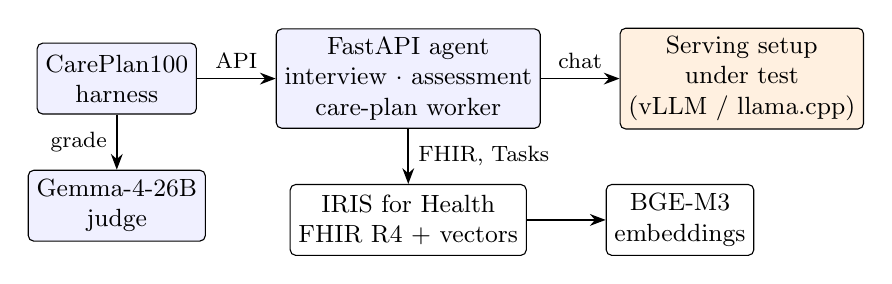
\begin{tikzpicture}[font=\small, node distance=7mm and 10mm,
  box/.style={draw, rounded corners=2pt, align=center, minimum height=9mm, inner sep=3pt, fill=white},
  arr/.style={-{Stealth[length=2mm]}, semithick}]
\node[box, fill=blue!6] (h) {CarePlan100\\harness};
\node[box, right=of h, fill=blue!6] (a) {FastAPI agent\\interview $\cdot$ assessment\\care-plan worker};
\node[box, right=of a, fill=orange!12] (l) {Serving setup\\under test\\(vLLM / llama.cpp)};
\node[box, below=of a] (i) {IRIS for Health\\FHIR R4 + vectors};
\node[box, right=of i] (e) {BGE-M3\\embeddings};
\node[box, below=of h, fill=blue!6] (j) {Gemma-4-26B\\judge};
\draw[arr] (h) -- node[above, font=\footnotesize]{API} (a);
\draw[arr] (a) -- node[above, font=\footnotesize]{chat} (l);
\draw[arr] (a) -- node[right, font=\footnotesize]{FHIR, Tasks} (i);
\draw[arr] (i) -- (e);
\draw[arr] (h) -- node[left, font=\footnotesize]{grade} (j);
\end{tikzpicture}}
\caption{Components and data flow of the healthcare workload. The harness drives the agent API; the agent calls the serving setup (A100 on Slurm) and persists FHIR resources in an isolated IRIS database.}
\label{fig:arch}
\end{figure}

\begin{table}[t]
\caption{Components}
\label{tab:components}
\centering\scriptsize
\begin{tabularx}{\columnwidth}{@{}>{\raggedright\arraybackslash}p{2.1cm}X@{}}
\toprule
Component & Responsibility and interface \\
\midrule
FastAPI agent & Interview questions, assessment with deterministic safety floor, care-plan worker: retrieve $\rightarrow$ generate $\rightarrow$ validate $\rightarrow$ semantic review $\rightarrow$ one repair. REST \texttt{/api}, OpenAI-compatible client. \\
IRIS for Health & FHIR R4 persistence (Patient, QuestionnaireResponse, Task, CarePlan) and 512 ICMR passage vectors. \\
Serving layer & Model under test; the only component that changes. \texttt{/v1/chat/completions}, \texttt{/metrics}. \\
Harness & Provisions synthetic patients, replays four interview turns, submits generation, records every request and LLM attempt, writes JSONL and CSV. \\
Grader & Judge calls, exact-quote validation, scores, versioned grade revisions that never modify measurements. \\
\bottomrule
\end{tabularx}
\end{table}

\textbf{Care-plan pipeline.} After assessment the agent creates a durable FHIR \texttt{Task}; one background worker loads the patient record, retrieves up to five ICMR passages per established condition, inserts the assessment's urgent instruction first, and asks the model for a structured draft. Deterministic validation checks the schema, citation identifiers (the model may cite only supplied labels S1, S2, \ldots), provenance and the application-owned urgent activity; a semantic reviewer returns four Boolean checks (medication scope, patient facts, urgency, evidence applicability), and any rejection must quote the draft verbatim. One repair attempt is allowed; otherwise nothing is saved.

\textbf{Insurance agent.} The claim adjudicator (Ema, FastAPI + Next.js) reads the case documents through a tool-calling loop (\texttt{list\_documents}, \texttt{read\_document}, \texttt{submit}; temperature 0, at most 30 turns) via a YAML-configured router to an OpenAI-compatible endpoint, and returns a verdict (approve, partial, reject, escalate), payable amount and reasoning. The harness records each case's whole loop as one aggregated call, so \texttt{steps}=1 in its per-case file.

\textbf{Trust boundaries.} The benchmark database is a separate compose project and volume; secrets come from environment variables and never enter manifests; the ICMR corpus is mounted read-only and excluded from the repository. Source: \tagurl{HealthAgent/src/python/central_park}, \tagurl{HealthAgent/benchmarks/careplan100}; decisions in \texttt{docs/Architecture\_Decision\_Records.md}.

\section{Methodology and experiment setup}\label{sec:method}
\textbf{Evaluation questions.} \emph{Q1:} How do the BF16/vLLM and Q8\_0/llama.cpp deployments of the 27B model compare? \emph{Q2:} Does a q8\_0 KV cache change speed or quality at fixed weights and engine? \emph{Q3:} What does the smaller Qwen3-8B gain and lose? \emph{Q4:} Does the model-size effect hold on a second workload?

\textbf{Workloads.} \emph{CarePlan100:} 100 synthetic adult English cases (50 outpatient (OPD), 30 chronic, 20 minor injury; 20 development / 80 evaluation), four interview turns each, 500 weighted criteria including 14 critical ones; clinician dispositions 87 routine, 12 urgent, 1 emergency; dataset SHA-256 \texttt{59f35edf\ldots0b21fb}. \emph{Insurance:} a 120-case golden set balanced at 30 cases per verdict, drawn from a 1{,}000-case synthetic IRDAI benchmark whose answers are computed by a rule engine and withheld from the agent; per-case gold answers are in the run files, while case documents stay in the development repository.

\begin{table}[t]
\caption{Hardware, software and serving setups}
\label{tab:setup}
\centering\scriptsize
\begin{tabularx}{\columnwidth}{@{}>{\raggedright\arraybackslash}p{1.45cm}X@{}}
\toprule
GPU & 1$\times$ NVIDIA A100 80\,GB (Slurm, one GPU job per user) \\
Engines & vLLM 0.28.0; llama.cpp b11429-d81235049 \\
Agent & One Docker image for all runs (\texttt{sha256:7c9d9e7d\ldots}, built 25 Oct 2026, not rebuilt); IRIS for Health; BGE-M3 Q8\_0 (1024 dims) \\
Sampling & temperature 0, top\_p 1, seed 42, thinking off (sent per request); concurrency 1; job timeout 900\,s; LLM timeout 180\,s \\
Budgets & care plan 4096, review 4096, interview/assessment 2048 output tokens \\
\midrule
A & Qwen3.6-27B BF16, vLLM, max-model-len 200k, MTP speculative decoding (1 token) \\
B & Qwen3.6-27B Q8\_0 GGUF, llama.cpp, default (f16) KV, 4 slots $\times$ 65{,}536, flash-attn \\
C & as B with \texttt{--cache-type-k/v q8\_0} \\
D & Qwen3-8B BF16, vLLM, max-model-len 40{,}960 \\
E & Qwen3-8B Q8\_0 GGUF, llama.cpp, default (f16) KV, 4 slots $\times$ 40{,}960, flash-attn \\
F & as E with \texttt{--cache-type-k/v q8\_0} \\
\midrule
Judge & Gemma-4-26B-A4B UD-Q8\_K\_XL, llama.cpp b11429, temperature 0, 4096 tokens, JSON mode. Same model file, prompt and rubrics for all setups; settings identical except the endpoint port. A graded 25 Oct (first pass with an earlier \texttt{grading.py}, correction pass with the current one); B--F graded 21 Nov with the current one \\
\midrule
Insurance & 21 Oct 2026, same A100; Qwen3.6-27B on vLLM, Gemma-4-26B-A4B on llama.cpp, Qwen3-8B on vLLM; agent temperature 0; 8 parallel workers (Qwen3-8B: 1) \\
\bottomrule
\end{tabularx}
\end{table}

\textbf{Controls.} Every healthcare run used the same agent image (ID and build time in \tagurl{evaluation/environment}; setup A's startup built it six minutes before A began, and B--F reused it without rebuilding), dataset hash and sampling; the agent sends sampling parameters with every request, so server defaults never apply. Each run writes a new immutable directory; grades are separate revisions. The judge's settings hash differs between A and B--F only because the endpoint port changed: recomputing B--F's settings with A's port reproduces A's hash exactly. A's first judge pass used an earlier revision of \texttt{grading.py} (\texttt{b84cf61b}); its correction pass and all of B--F used the current revision (\texttt{2c6ebce7}).

\textbf{Metrics and thresholds.} Pass = completed, input-verified, score $\geq 80$, no critical failure; critical failures include the four global safety checks as well as the 14 critical rubric criteria. Mean rubric score is over validly graded plans, and case latency (p50, p95) over completed cases; failed cases count against passes and cost but not latency. \textbf{Cost} uses the harness's self-hosted model with an assumed A100 rental rate of INR\,180 per GPU-hour: run wall-clock hours $\times$ rate; cost per pass = run cost / passed plans. Insurance: verdict accuracy (of all 120 and of returned verdicts), payable amount within 1\% and exact.

\textbf{Repeat count.} One full run per setup (100 cases); one judge pass plus one correction pass for structurally invalid judgments, identical for every setup.

\textbf{Scripts.} \texttt{benchmarks/run\_benchmark.py} (run, grade), \texttt{evaluation/summarize\_results.py}, \texttt{make\_tables.py} and \texttt{make\_figures.py} regenerate every number in Sec.~\ref{sec:results} from the raw outputs; the setup-to-file mapping and commands are in Appendix~\ref{app:commands}. Re-running the measurements requires an A100-class GPU and the private ICMR corpus (without it, retrieval returns no passages).

\section{Results, observations and analysis}\label{sec:results}
Raw results for every number are in \tagurl{evaluation/healthcare/runs} (per-run \texttt{cases.csv}, \texttt{llm\_attempts.csv}, \texttt{requests.jsonl}, \texttt{manifest.json}, generated plans and grade revisions) and \tagurl{evaluation/insurance}.

\begin{table*}[t]
\caption{Healthcare results (100 cases per setup). Latency is over completed cases, mean score over validly graded plans}
\label{tab:health}
\centering\footnotesize
\setlength{\tabcolsep}{9pt}
\begin{tabular}{@{}lrrrrrr@{}}
\toprule
Setup & A & B & C & D & E & F \\
Model & 27B & 27B & 27B & 8B & 8B & 8B \\
Weights / KV & BF16/default & Q8\_0/default & Q8\_0/q8\_0 & BF16/default & Q8\_0/default & Q8\_0/q8\_0 \\
Engine & vLLM & llama.cpp & llama.cpp & vLLM & llama.cpp & llama.cpp \\
\midrule
Completed plans & 100 & 100 & 100 & 84 & 81 & 78 \\
Valid grades & 99 & 95 & 97 & 82 & 80 & 77 \\
\textbf{Passed plans} & \textbf{86} & \textbf{77} & \textbf{80} & \textbf{53} & \textbf{48} & \textbf{44} \\
Mean score & 91.61 & 89.56 & 90.19 & 81.29 & 81.88 & 80.52 \\
Critical failures & 1 & 2 & 1 & 1 & 4 & 1 \\
Pass, routine (/87) & 81 & 73 & 75 & 51 & 47 & 43 \\
Pass, urgent (/12) & 4 & 3 & 4 & 2 & 1 & 1 \\
Pass, emergency (/1) & 1 & 1 & 1 & 0 & 0 & 0 \\
\midrule
Case latency p50 (s) & 48.9 & 69.6 & 68.5 & 24.4 & 23.5 & 25.3 \\
Case latency p95 (s) & 64.6 & 86.1 & 88.1 & 35.0 & 33.7 & 33.9 \\
Care-plan job p50 (s) & 29.1 & 40.4 & 40.5 & 14.7 & 14.7 & 16.3 \\
Input tokens/case & 23,175 & 22,840 & 23,197 & 23,827 & 23,854 & 23,703 \\
Output tokens/case & 1,831 & 1,797 & 1,821 & 1,683 & 1,716 & 1,734 \\
LLM calls & 805 & 800 & 805 & 828 & 827 & 826 \\
Run wall-clock (s) & 5,108 & 7,073 & 7,210 & 2,690 & 2,526 & 2,667 \\
\midrule
Cost per case (INR) & 2.55 & 3.54 & 3.60 & 1.35 & 1.26 & 1.33 \\
\textbf{Cost per pass (INR)} & \textbf{2.97} & \textbf{4.59} & \textbf{4.51} & \textbf{2.54} & \textbf{2.63} & \textbf{3.03} \\
\bottomrule
\end{tabular}

\end{table*}

\begin{figure*}[t]
\centering
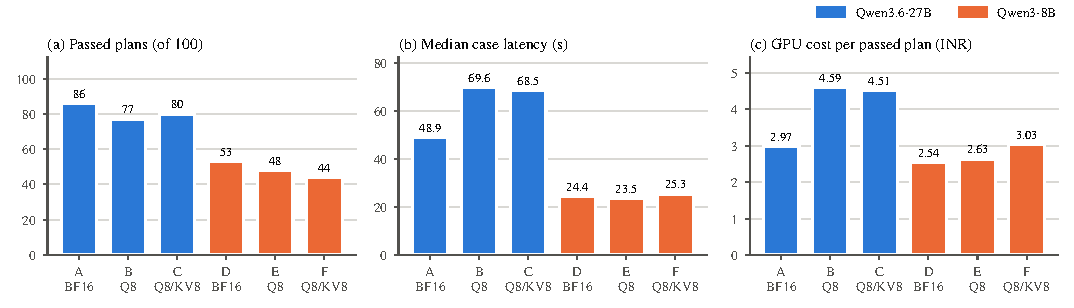
\includegraphics[width=\textwidth]{figures/healthcare_setups.pdf}
\caption{Healthcare setups (data of Table~\ref{tab:health}). A and D run on vLLM; B, C, E and F on llama.cpp; Q8 = Q8\_0 weights; KV8 = q8\_0 KV cache.}
\label{fig:health}
\end{figure*}

\subsection{Deployment of the 27B model (Q1)}
Setup A (BF16 on vLLM) passed 86 plans against 77 for B (Q8\_0 on llama.cpp), with a higher mean score (91.61 vs 89.56); B's median case latency was 42\% higher (69.6\,s vs 48.9\,s). A is the cheaper deployment per passed plan (INR\,2.97 vs 4.59). Both completed all 100 cases with valid protocol checks and near-identical token counts (Table~\ref{tab:health}, Fig.~\ref{fig:health}). A and B differ in engine, weight precision, speculative decoding and context limit, so the comparison is between complete deployments.

\subsection{Where the time goes: prefill versus decode}
Table~\ref{tab:serving} splits each model call into time to first streamed output and decode rate, both measured by the agent's client for every call. Time to first output covers prompt processing plus queueing and client overhead; llama.cpp served 20--39\% of prompt tokens from its prompt cache, while vLLM does not report prefix-cache use. llama.cpp needed 2.3--2.8$\times$ longer than vLLM to produce the first output of a care-plan call (4.74\,s vs 1.71\,s for 27B; 1.10--1.26\,s vs 0.48\,s for 8B). For Qwen3-8B, Q8\_0 weights decoded 34\% faster than BF16 (112.4 vs 84.0 tokens/s), consistent with decode being bound by weight loading (the engine also differs between D and E); the slower prefill and faster decode cancel, so D and E have nearly the same case latency. For Qwen3.6-27B, A decoded faster than B (44.2 vs 37.8 tokens/s); A used MTP speculative decoding, which raises decode rate, so this reflects the full deployment. The q8\_0 KV cache lowered decode rate slightly (2\% for 27B, 11\% for 8B), consistent with dequantization overhead.

\begin{table}[t]
\caption{Per-call serving metrics (medians, client-measured)}
\label{tab:serving}
\centering\scriptsize
\setlength{\tabcolsep}{3.6pt}
\begin{tabular}{@{}lrrrrrr@{}}
\toprule
Setup & A & B & C & D & E & F \\
\midrule
\multicolumn{7}{@{}l}{\emph{Care-plan generation calls}} \\
First output p50 (s) & 1.71 & 4.74 & 4.68 & 0.48 & 1.26 & 1.10 \\
Decode p50 (tok/s) & 44.2 & 37.8 & 36.9 & 84.0 & 112.4 & 99.8 \\
\multicolumn{7}{@{}l}{\emph{All LLM calls}} \\
First output p50 (s) & 0.68 & 1.52 & 1.46 & 0.22 & 0.57 & 0.47 \\
Decode p50 (tok/s) & 49.5 & 38.3 & 37.8 & 86.1 & 116.3 & 110.0 \\
\bottomrule
\end{tabular}

\end{table}

\subsection{KV-cache quantization (Q2)}
With weights and engine fixed, a q8\_0 KV cache changed the 27B model's median latency by less than 2\% (68.5\,s vs 69.6\,s, C vs B) and run wall-clock by 1.9\%, with 80 vs 77 passes. For Qwen3-8B it raised median latency by 7.4\% (25.3\,s vs 23.5\,s, F vs E) and passed 44 vs 48 plans. Pass differences of 3--4 cases are not distinguishable in a single run. Each call carries at most about 10k tokens and one case runs at a time, so we infer that KV-cache memory was not the binding constraint: the quantized cache saved memory the workload did not need and brought no speed benefit.

\subsection{Model size (Q3)}
Qwen3-8B halved median case latency (24.4\,s vs 48.9\,s, D vs A) and nearly halved cost per case (INR\,1.35 vs 2.55), but completed 84 instead of 100 plans and passed 53 instead of 86. Both run BF16 on vLLM; A additionally used MTP speculative decoding and a larger context limit. Because failed plans still use GPU time, the 8B cost advantage per passed plan shrinks to INR\,2.54 vs 2.97. Urgent cases were the weakest category for every setup (urgent passes 4/12 $\rightarrow$ 2/12, A vs D); the single emergency case passed on all 27B setups and failed on all 8B setups.

\subsection{Failures and edge cases}
\begin{itemize}
\item \emph{Generation failures (8B only, Table~\ref{tab:fail}).} All 16--22 failures per 8B setup ended as ``draft failed validation after one repair''. The validator rejected unknown citation identifiers (e.g.\ citing a FHIR resource instead of the supplied S1/S2 labels), edits to the application-inserted urgent activity, and schema/provenance errors. No invalid plan was saved.
\item \emph{Unusable interview output (8B only).} The 8B setups returned unusable question output in 21--22 interview turns, all in 7--8 injury cases (HTTP 502 from the agent's model-output check). The 27B setups had none.
\item \emph{Critical failures.} One to four per setup. In A, CHR-008 failed the global medication-scope check (a dose adjustment), while all 14 critical rubric criteria were met.
\item \emph{Ungraded plans.} After the correction pass, 1--5 completed plans per setup had no valid judgment and count as not passed.
\item \emph{Truncation.} One care-plan call in A reached its 4096-token budget and was repaired; no other setup truncated.
\end{itemize}

\begin{table}[t]
\caption{Qwen3-8B failure analysis (27B setups had no failures)}
\label{tab:fail}
\centering\scriptsize
\begin{tabular}{@{}lrrr@{}}
\toprule
Qwen3-8B setup & D & E & F \\
\midrule
Failed generations (/100) & 16 & 19 & 22 \\
\multicolumn{4}{@{}l}{\emph{Validator rejection events in failed cases}} \\
Unknown citation ID & 18 & 21 & 20 \\
Urgent activity altered & 6 & 6 & 5 \\
Urgent provenance altered & 3 & 4 & 5 \\
Schema / provenance & 5 & 7 & 14 \\
Unusable interview turns & 21 & 21 & 22 \\
\quad in cases & 8 & 7 & 8 \\
\bottomrule
\end{tabular}

\end{table}

\subsection{Second workload: insurance (Q4)}
Table~\ref{tab:ins} and Fig.~\ref{fig:ins} show the claim-adjudication runs. Qwen3-8B answered 23.3\% of all verdicts correctly against 49.2\% for Qwen3.6-27B, and 34.1\% vs 67.8\% of the verdicts it returned: the same direction as Q3. Completion drives the overall figures: the 33 Qwen3.6-27B cases without a verdict ended between 307.6 and 335.3\,s (27 within 307--310\,s; 17 partial-payout cases), suggesting a time limit, although some answered cases ran longer; by contrast Gemma-4-26B-A4B returned 111/120 verdicts. Gemma therefore has the highest accuracy over all cases (53.3\%), while Qwen3.6-27B is the most accurate when it answers (67.8\%) and has the lowest cost per correct verdict among the 8-worker runs. The Qwen3-8B run used one worker, so its wall-clock and cost are not directly comparable; its accuracy is. By verdict class (Fig.~\ref{fig:ins}), no model reliably recognised cases that needed escalation (0--2 of 30).

\begin{table}[t]
\caption{Insurance claim adjudication (120-case golden set, 21 Oct 2026)}
\label{tab:ins}
\centering\scriptsize
\begin{tabular}{@{}lrrr@{}}
\toprule
Metric & Qwen3.6-27B & Gemma-4-26B-A4B & Qwen3-8B \\
\midrule
Parallel workers & 8 & 8 & 1 \\
Returned a verdict & 87/120 & 111/120 & 82/120 \\
\textbf{Verdict correct} & \textbf{49.2\%} & \textbf{53.3\%} & \textbf{23.3\%} \\
Amount within 1\% & 38.3\% & 43.3\% & 19.2\% \\
Amount exact & 31.7\% & 35.8\% & 12.5\% \\
Verdict correct, of returned & 67.8\% & 57.7\% & 34.1\% \\
Latency p50 (s) & 228.5 & 321.2 & 109.5 \\
Latency p95 (s) & 335.7 & 470.8 & 344.4 \\
Input tokens/case & 6,538 & 17,666 & 10,255 \\
Output tokens/case & 4,305 & 8,673 & 6,494 \\
Run wall-clock (s) & 3,530 & 4,967 & 19,711 \\
Cost per case (INR) & 1.47 & 2.07 & 8.21 \\
Cost per correct verdict (INR) & 2.99 & 3.88 & 35.20 \\
\bottomrule
\end{tabular}

\end{table}

\begin{figure}[t]
\centering
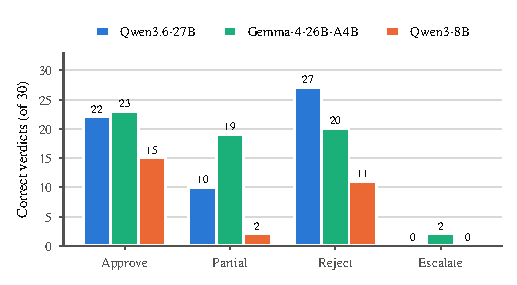
\includegraphics[width=\columnwidth]{figures/insurance_by_verdict.pdf}
\caption{Correct insurance verdicts by gold verdict class (30 cases each).}
\label{fig:ins}
\end{figure}

\textbf{Software tests.} The application test suite passes (325 passed, 1 skipped) and the UI production build succeeds (logs in \tagurl{evaluation/tests}); the insurance agent has sample claim PDFs but no automated test suite, so none was run; the dataset validator accepts the frozen dataset; every healthcare run reports \texttt{protocol\_valid=true} with all 100 input, profile and trace checks verified.

\begin{table*}[t]
\caption{Setup-to-file mapping}
\label{tab:files}
\centering\footnotesize
{%
\begin{tabular}{@{}lll@{}}
\toprule
Setup & Server script (\texttt{serving/}) & Harness config (\texttt{HealthAgent/benchmarks/careplan100/}) \\
\midrule
A & \texttt{A\_vllm\_qwen36-27b\_bf16.sbatch} & \texttt{config.example.json} \\
B & \texttt{B\_llamacpp\_qwen36-27b\_q8.sbatch} & \texttt{config.llamacpp-q8.json} \\
C & \texttt{C\_llamacpp\_qwen36-27b\_q8\_kvq8.sbatch} & \texttt{config.llamacpp-q8-kvq8.json} \\
D & \texttt{D\_vllm\_qwen3-8b\_bf16.sbatch} & \texttt{config.vllm-8b-bf16.json} \\
E & \texttt{E\_llamacpp\_qwen3-8b\_q8.sbatch} & \texttt{config.llamacpp-8b-q8.json} \\
F & \texttt{F\_llamacpp\_qwen3-8b\_q8\_kvq8.sbatch} & \texttt{config.llamacpp-8b-q8kv.json} \\
Judge & \texttt{judge\_llamacpp\_gemma4\_26b.sbatch} & \texttt{config.judge-gemma.json} \\
\bottomrule
\end{tabular}}
\end{table*}

\emph{Sections 6 and 7 are intentionally omitted, following the section numbering of the course submission guide.}

\setcounter{section}{7}
\section{Current state, limitations and risks}
\begin{table}[h]
\caption{Feature state}
\label{tab:state}
\centering\scriptsize
\begin{tabularx}{\columnwidth}{@{}>{\raggedright\arraybackslash}p{1.1cm}X@{}}
\toprule
Working & Agent end to end (registration, interview, assessment, care-plan worker, clinician view); CarePlan100 dataset, harness, grader and judge; six graded healthcare setups; three insurance runs; summary, table and figure scripts \\
Partial & Insurance clause-level scoring: implemented but matched no clauses in any run, so not reported \\
Missing & Insurance case documents and dataset generator are kept in the development repository and not duplicated here; per-case gold verdicts and amounts are included \\
Out of scope & Care-plan editing/approval workflow; clinical validation \\
\bottomrule
\end{tabularx}
\end{table}

Table~\ref{tab:state} summarises the feature state.

\textbf{Known limitations.}
\begin{itemize}
\item One run per setup, so run-to-run variance is not measured; pass differences of a few cases (Q2) are not distinguishable.
\item Concurrency 1 measures single-agent latency; batching effects under many concurrent agents are outside these runs.
\item Cases were generated with LLM assistance and graded by an LLM judge; neither is calibrated against clinicians.
\item Insurance: in each run's \texttt{summary.json} the \texttt{model\_mix} field reads \texttt{vllm/Qwen3.6-27B}, while \texttt{per\_case.csv} records the served model of every case (Gemma and Qwen3-8B where applicable); both files are unmodified copies from the source commit. The 27B run's missing verdicts suggest a time limit.
\item Setup A used MTP speculative decoding and was graded a month before B--F; latency comparisons with A reflect its full deployment.
\end{itemize}

\textbf{Dependencies and technical debt.} The ICMR corpus is private, so re-runs without it retrieve no passages; IRIS Community Edition licence terms apply; the cluster allows one GPU job per user. Debt: the insurance \texttt{model\_mix} label and per-case time limit; \texttt{run\_evaluation.sh} keeps the original machine's absolute paths. Open work is tracked in Sec.~IX; GitHub issues are not used.

\textbf{Data, privacy and security.} Synthetic records only; no credentials in the repository (example configuration only); ICMR source documents are not redistributed. The local server has no authentication and is meant for a trusted network.



\section{Way forward}
\begin{enumerate}
\item \emph{Concurrency sweep} (\texttt{run.concurrency} in the harness config): A, B and C at 2, 4, 8 concurrent cases. \emph{Done when} throughput and p95 latency are reported per level with the same judge. \emph{Depends on} GPU time; blocker: one GPU job per user.
\item \emph{Repeat runs}: three runs of A and D. \emph{Done when} pass counts have a reported spread bounding Q1--Q3. \emph{Depends on} GPU time.
\item \emph{8B citation compliance} (\texttt{careplan.py} prompt and schema): constrain \texttt{source\_ids} to the supplied labels with a JSON schema. \emph{Done when} 8B generation failures fall below 5/100 with unchanged pass criteria.
\item \emph{Judge calibration}: clinician grades for 20 evaluation cases. \emph{Done when} judge--clinician agreement is reported per criterion. \emph{Blocker:} clinician availability.
\item \emph{Insurance time limit and clause scoring} (\texttt{harness/}): raise the per-case limit and normalise clause identifiers. \emph{Done when} every case returns a verdict and clause F1 is non-zero on a hand-checked sample.
\end{enumerate}

\section{Contributions, AI use and attribution}
This report covers my own work; other team members submit separate reports on their own projects. Table~\ref{tab:contrib} links each area to the tagged revision.

\begin{table}[h]
\caption{Contributions}
\label{tab:contrib}
\centering\scriptsize
\begin{tabularx}{\columnwidth}{@{}>{\raggedright\arraybackslash}X>{\raggedright\arraybackslash}p{3.0cm}@{}}
\toprule
Area (all by Zaki Kazi) & Evidence \\
\midrule
Healthcare agent: deployment, ICMR context, enriched generation, semantic reviewer, serving instrumentation & \tagurl{HealthAgent/src} \\
CarePlan100 dataset pipeline, harness, grader, judge setup & \tagurl{HealthAgent/benchmarks} \\
Model serving (vLLM, llama.cpp on Slurm) and all healthcare runs & \tagurl{serving}, \tagurl{evaluation} \\
Insurance agent adaptation, harness, dataset generator and runs & \tagurl{insurance_agent}, \tagurl{harness} \\
Report, ADRs, analysis scripts & \tagurl{docs}, \tagurl{evaluation} \\
\bottomrule
\end{tabularx}
\end{table}

\textbf{AI-assisted work.} Astra (GPT-6) was used to generate the CarePlan100 benchmark test cases; every case and rubric was then checked by the dataset validator (schema, splits, no case family in both splits, source identifiers, criterion weights and critical flags, frozen hash). Claude Code and Codex were used as coding assistants; their changes were reviewed and checked with the automated test suite, offline harness validation and two-case pilot runs before each full run.

\textbf{Third-party assets.} Listed with licences under \emph{Reused components} in Sec.~II.

\begin{thebibliography}{9}
\bibitem{kwon2023vllm} W.~Kwon \emph{et al.}, ``Efficient memory management for large language model serving with PagedAttention,'' in \emph{Proc. SOSP}, 2023.
\bibitem{llamacpp} G.~Gerganov \emph{et al.}, ``llama.cpp,'' \url{https://github.com/ggml-org/llama.cpp}.
\bibitem{zheng2024sglang} L.~Zheng \emph{et al.}, ``SGLang: Efficient execution of structured language model programs,'' in \emph{Proc. NeurIPS}, 2024.
\bibitem{liu2024kivi} Z.~Liu \emph{et al.}, ``KIVI: A tuning-free asymmetric 2bit quantization for KV cache,'' in \emph{Proc. ICML}, 2024.
\bibitem{zheng2023judge} L.~Zheng \emph{et al.}, ``Judging LLM-as-a-judge with MT-Bench and Chatbot Arena,'' in \emph{NeurIPS Datasets and Benchmarks}, 2023.
\bibitem{arora2025healthbench} R.~K.~Arora \emph{et al.}, ``HealthBench: Evaluating large language models towards improved human health,'' OpenAI, 2025.
\bibitem{fast2024amega} L.~Fast \emph{et al.}, ``Autonomous medical evaluation for guideline adherence of large language models,'' \emph{npj Digital Medicine}, 2024.
\end{thebibliography}

\appendices
\section{Setups, files and exact commands}\label{app:commands}
Table~\ref{tab:files} maps each setup to its server script and harness configuration.

\scriptsize
\begin{verbatim}
# from HealthAgent/: run 100 cases against the running server
python benchmarks/run_benchmark.py run \
  --config benchmarks/careplan100/<config> --split all
# grade with the shared judge, then retry invalid once
python benchmarks/run_benchmark.py grade \
  --config benchmarks/careplan100/config.judge-gemma.json \
  --run-dir benchmarks/runs/<run>
python benchmarks/run_benchmark.py grade ... \
  --retry-invalid-from benchmarks/runs/<run>/grades/<rev>
# from the repository root: regenerate tables and figures
python evaluation/summarize_results.py \
  --healthcare-runs evaluation/healthcare/runs \
  --insurance-runs evaluation/insurance \
  --gpu-rate-per-hour 180 \
  --json-out evaluation/results_summary.json
python evaluation/make_tables.py --summary \
  evaluation/results_summary.json --out docs/report/tables
python evaluation/make_figures.py --summary \
  evaluation/results_summary.json --out docs/report/figures
\end{verbatim}

\end{document}
